\documentclass[conference]{IEEEtran}
\IEEEoverridecommandlockouts
\usepackage{cite}
\usepackage{amsmath,amssymb,amsthm}
\usepackage{booktabs}
\usepackage{graphicx}
\usepackage{hyperref}
\usepackage{url}

\newtheorem{theorem}{Theorem}
\newtheorem{lemma}{Lemma}
\newtheorem{corollary}{Corollary}
\newtheorem{definition}{Definition}
\newtheorem{assumption}{Assumption}

\title{An Analytical Feasibility Study of Post Quantum Sizing, ZKML Soundness, and Trust Scoring for Proof of Useful Intelligence Consensus}

\author{
\IEEEauthorblockN{Md.\ Mehedi Hasan, Asraful Islam Sharthak, Prof.\ Dr.\ Md.\ Abdul Based}
\IEEEauthorblockA{\textit{Dhaka International University}\\
Dhaka, Bangladesh}

}

\begin{document}
\maketitle

\begin{abstract}

Proof of useful intelligence (PoUI) proposes using AI computation as useful work in a consensus design. A deployable system must define how validators are scored, how claimed computations are verified, and how cryptographic messages fit within a block budget. This paper presents an analytical feasibility study, not a blockchain implementation. We analyze a trust score, derive score bounds and an expected score gap, examine a one-agent score-maximization result under stated assumptions, and derive geometric exclusion time under an independent audit model. In a 100-node simulation using sampled accuracy and latency proxies and assuming zero honest false positives, all 15 malicious nodes were excluded in each of ten seeds. The mean of the per-seed mean exclusion epochs was $3.12$ (standard deviation $0.71$), compared with the model prediction $1/0.35\approx2.86$. We sketch a challenge/proof/score flow, list five ZKML circuit review questions, and report FIPS/RFC parameter sizes and illustrative payload arithmetic. A tiny EZKL proof-pipeline run is a smoke test, not a production audit or benchmark. No consensus network or local PQC primitive benchmark is implemented.
\end{abstract}

\begin{IEEEkeywords}
Blockchain consensus, ML-DSA, ML-KEM, ZKML, underconstrained circuits, trust score, and proof of useful intelligence
\end{IEEEkeywords}

\section{Introduction}
\label{sec:intro}

Proof of work expends energy on a search whose purpose is consensus~\cite{nakamoto2008}; proof of stake instead uses capital at risk~\cite{saleh2021pos}. Research on useful proof of work~\cite{lihu2020pouw,baldominos2019coinai} and proof of useful intelligence (PoUI)~\cite{chong2025poui} explores using computation for machine learning tasks as consensus work. Bittensor is a deployed market for model outputs that uses peer scoring within subnets~\cite{bittensor2024}; this paper instead studies requirements for linking a score to a verifiable computation.

If PoUI is going to be used as a consensus rule, three engineering problems come up at once.

\begin{enumerate}
  \item \textbf{Scoring.} Accuracy, latency, and uptime must be combined into a score. This study does not model identity splitting or demonstrate resistance to false outputs that evade a real audit.
  \item \textbf{Proof soundness.} A SNARK or comparable evidence that "the model ran" is only as reliable as the circuit. In general purpose ZK systems, underconstrained circuits are a known class of bugs~\cite{pailoor2023pldi}, neural network devices (ReLU, ArgMax, quantized softmax) add more ways to cheat.
  \item \textbf{Post quantum bytes.} FIPS 204 signatures are significantly larger than Ed25519~\cite{nistfips204,rfc8032}. Replacing validator signatures without considering block size is not recommended.
\end{enumerate}

\paragraph{Research topic and methodology}
What verification and message-budget requirements must accompany a PoUI trust score, and under what explicit assumptions can it exclude low-quality reports? We address this question with (i) an analysis of a score and audit model, (ii) a reproducible Monte Carlo that compares sampled outcomes with the model's exclusion-time prediction, and (iii) a review of post-quantum interfaces and ZKML design considerations. This is an analysis of requirements and feasibility, not an implementation or a head-to-head consensus benchmark.

\paragraph{Contributions}
\begin{itemize}
  \item \textbf{Analytical trust score model.} We provide bounds, an expected score gap, a one agent score maximization result, and a geometric exclusion time theorem under specific audit and independence assumptions. The maximization result does not establish truthful reporting.
  \item \textbf{Model consistency check.} Across ten seeds, the mean of the per seed mean exclusion epochs is $3.12$ (standard deviation $0.71$), compared with the model prediction of $2.86$. This is a sanity check, not independent security validation.
 \item \textbf{Protocol and implementation considerations.} We sketch a challenge/proof/score flow, list five ZKML circuit review questions, and discuss FIPS 204 parameter sizes and cross layer design risks.
  \item \textbf{ZKML pipeline smoke test.} We run a deterministic two-input affine ReLU ONNX model through EZKL setup, proving, and verification. This demonstrates a local toolchain path, not a benchmark for a useful model.
\end{itemize}

\paragraph{Evaluation boundary}
The simulator does not train or execute a neural model, exchange network messages, or measure PQC operations. The small EZKL run is a toolchain smoke test, not an EZKL/Halo2 audit or general performance result. The vote baseline is a toy rule: its $0.02$ exclusion probability applies only after a malicious validator is selected for a 10 member committee. It is not representative of proof of stake protocols.
\section{Related Work}
\label{sec:related}

Chong et al.\ present PoUI as an integration of AI work with staking~\cite{chong2025poui}. This study analyzes a score and exclusion threshold under an explicit audit model. Lihu et al.\ and Baldominos and Saez incorporate training or inference within the mining loop~\cite{lihu2020pouw,baldominos2019coinai}. DeepChain examines collaborative learning with incentives and on-chain audit trails~\cite{weng2021deepchain}. Bittensor is a related deployed market whose scoring relies on peer evaluation within subnets~\cite{bittensor2024}.
Groth's SNARK and PLONK backends are commonly used in proofs~\cite{groth2016,plonk2019}. Pailoor et al.\ (PLDI 2023) developed an automated method for identifying underconstrained circuits~\cite{pailoor2023pldi}. Peng et al.\ conducted a survey on verifiable machine learning, including cost and quantification~\cite{peng2025zkml}. EZKL builds ONNX style graphs into circuits~\cite{ezkl2024}. Worldcoin employs zero knowledge proofs for biometric uniqueness, a distinct threat model from validator inference~\cite{worldcoin2023}.

NIST standardized ML-KEM and ML-DSA in 2024~\cite{nistfips203,nistfips204}. Baseri et al.\ evaluated ledger migration risks during quantum attacks~\cite{baseri2025quantum}. These works motivate considering cryptographic payloads alongside the timing and byte budgets of a proof-intensive PoUI slot.
This work connects these strands at the requirement level.
The score indicates what should be measured, the circuit determines what can be trusted, and the PQC payload must fit within the protocol's timing and byte budgets.

\section{Threat Model and Scope}
\label{sec:threat}

The model considers a validator set of size $N$. Each epoch $t$, a node has an inference accuracy proxy $A_t\in[0,1]$, latency $L_t\geq0$ (ms), uptime ratio $U_t\in(0,1]$, and slash bit $S_t\in\{0,1\}$. Honest accuracy is drawn from a Gaussian clipped to $[0,1]$, latency is drawn from a normal distribution floored at $1$ ms. High latency nodes receive an additional $30$ ms. Malicious accuracy is drawn uniformly from $[0.10,0.30]$, when $A_t<\tau=0.40$, a node is independently slashed with probability $p_{\mathrm{detect}}=0.35$. Honest nodes are never slashed in this model, this zero false positive assumption is optimistic.

The model focuses on low-quality reports whose accuracy falls below the audit threshold. It does not model identity creation costs, identity splitting, or stake-weighted selection and therefore does not establish Sybil resistance.

The simulator does not call a ZKML system. Section~\ref{sec:zkml}'s checklist identifies questions for a future circuit; it does not measure an assembled graph.

Key and signature sizes are taken from the cited standards. The repository script calculates parameter sizes and illustrative payloads; it does not measure cryptographic operation timings.

\section{Trust Score}
\label{sec:trust}

\begin{definition}[Trust score]
For epoch $t\in\mathbb{N}$,
\begin{equation}
  T_t = \alpha A_t^2 e^{-\lambda L_t} + \beta \ln U_t - \gamma S_t,
  \label{eq:trust}
\end{equation}
with weights $\alpha,\beta,\gamma,\lambda>0$. Experiments use $\alpha=0.5$, $\beta=0.3$, $\gamma=1.5$, $\lambda=0.01$. A node leaves the active set when $T_t < \tau_{\mathrm{excl}}=-0.5$. Implementations should floor $U_t$ at $\epsilon_U>0$ so that $\ln U_t$ is finite, the simulator uses $\max(U_t,10^{-9})$.
\end{definition}

\begin{assumption}[Independence and audits]
\label{ass:ind}
$A_t$ and $L_t$ are independent. Honest nodes have $S_t=0$. A low-quality report with $A_t<\tau$ is slashed independently with probability $p\in(0,1]$; if $A_t\ge\tau$, then $S_t=0$. (The simulator assumes $\tau=0.40$ and $p=0.35$.)
\end{assumption}

\begin{theorem}[Bounds]
\label{thm:bounds}
If $A_t\in[0,1]$, $L_t\ge 0$, $U_t\in[\epsilon_U,1]$, and $S_t\in\{0,1\}$, then
\[
  \beta\ln\epsilon_U-\gamma \le T_t \le \alpha.
\]
The upper bound is attained at $(A_t,L_t,U_t,S_t)=(1,0,1,0)$. If the protocol enforces $L_t\ge L_{\min}>0$, the bound tightens to $T_t\le\alpha e^{-\lambda L_{\min}}$.
\end{theorem}

\begin{proof}
Because $A_t^2\le 1$ and $e^{-\lambda L_t}\le 1$, the accuracy term is at most $\alpha$, with equality only if $A_t=1$ and $L_t=0$. Because $\ln U_t\le\ln 1=0$, the uptime term is at most $0$, with equality only if $U_t=1$. Because $S_t\ge 0$, $-\gamma S_t\le 0$, with equality only if $S_t=0$. Adding these three inequalities yields $T_t\le\alpha$. For the lower bound, the accuracy term is $\ge 0$, $\ln U_t\ge\ln\epsilon_U$, and $-\gamma S_t\ge-\gamma$. If $L_t\ge L_{\min}$, then $e^{-\lambda L_t}\le e^{-\lambda L_{\min}}$, so the first term is at most $\alpha e^{-\lambda L_{\min}}$.
\end{proof}

Write $\phi_L:=\mathbb{E}[e^{-\lambda L_t}]$. Independence in Assumption~\ref{ass:ind} gives $\mathbb{E}[A_t^2 e^{-\lambda L_t}]=\mathbb{E}[A_t^2]\,\phi_L$. We do \emph{not} replace $\phi_L$ by $e^{-\lambda\mathbb{E}[L_t]}$ (Jensen would go the wrong way for the convex map $x\mapsto e^{-\lambda x}$ on $\lambda>0$).

\begin{theorem}[Expected score gap]
\label{thm:score gap}
Under Assumption~\ref{ass:ind}, set $U_t=1$ for both kinds and apply the latency law that defines $\phi_L$. Assume an honest node has accuracy $A_H$ and a fabricator reports a (potentially random) $A_F$ with $A_F<\tau$ a.s.\ and $\mathbb{E}[S_F]=p$. Then
\begin{equation}
  \Delta := \mathbb{E}[T_H]-\mathbb{E}[T_F]
  = \alpha\phi_L\bigl(\mathbb{E}[A_H^2]-\mathbb{E}[A_F^2]\bigr)+\gamma p.
  \label{eq:gap}
\end{equation}
In particular $\Delta>0$ whenever $\gamma p>\alpha\phi_L\bigl(\mathbb{E}[A_F^2]-\mathbb{E}[A_H^2]\bigr)_+$, which holds automatically if $\mathbb{E}[A_H^2]\ge\mathbb{E}[A_F^2]$.
\end{theorem}

\begin{proof}
$\mathbb{E}[T_H]=\alpha\mathbb{E}[A_H^2]\phi_L$ because $S_H=0$ and $\ln 1=0$. $\mathbb{E}[T_F]=\alpha\mathbb{E}[A_F^2]\phi_L-\gamma p$. Subtract.
\end{proof}

The expected score gap compares individual score distributions under the assumptions above. It does not model identity multiplication, stake allocation, or validator selection and therefore does not establish Sybil resistance.

The formal analysis script uses $\phi_L=\mathbb{E}[e^{-0.01 L}]$ for latency drawn from a normal distribution with mean $50$ ms and standard deviation $10$ ms, floored at $1$ ms. Under the script's clipped honest accuracy distribution and the simulator's $A_F\sim\mathrm{Unif}[0.10,0.30]$ fabricator distribution, the model derived expected score gap is approximately $0.75917$. This is an analytical result under the stated assumptions, not a measured performance result.

\begin{theorem}[Unique maximizer of the one shot payoff]
\label{thm:game}
Fix $L_t$ and $U_t$, and let $\mathbb{E}[S_t\mid A]=p\cdot\mathbf{1}[A<\tau]$ as in Assumption~\ref{ass:ind}. Define $g(A)=\alpha A^2 e^{-\lambda L_t}+\beta\ln U_t-\gamma p\cdot\mathbf{1}[A<\tau]$ for $A\in[0,1]$. If $\tau\in(0,1]$ and $p,\alpha,\gamma>0$, then $g$ has a unique maximizer at $A=1$.
\end{theorem}

\begin{proof}
Let $c:=\alpha e^{-\lambda L_t}>0$ and $b:=\beta\ln U_t$, so $g(A)=cA^2+b-\gamma p$ on $[0,\tau)$ and $g(A)=cA^2+b$ on $[\tau,1]$. Since $\tau\le 1$, $g(1)=c+b$. For any $A<1$ we have $cA^2<c$, hence $g(A)<c+b-\gamma p\,\mathbf{1}[A<\tau]\le c+b=g(1)$. Every $A<1$ is therefore strictly worse than $A=1$.
\end{proof}

This is a single agent optimization, not a Nash equilibrium in a repeated game with stakes or collusion. The simulator does not compare a reported accuracy with hidden ground truth, so the maximizer does not establish truthful reporting.

\begin{lemma}[One slash suffices]
\label{lem:slash}
Assume $U_t=1$, $\tau_{\mathrm{excl}}<0$, and $\gamma>\alpha-\tau_{\mathrm{excl}}$. Then $S_t=0$ implies $T_t\ge 0>\tau_{\mathrm{excl}}$ (using $A_t^2 e^{-\lambda L_t}\ge 0$), while $S_t=1$ implies $T_t\le\alpha-\gamma<\tau_{\mathrm{excl}}$. Thus exclusion occurs if and only if $S_t=1$.
\end{lemma}

The experimental parameters satisfy $\alpha-\tau_{\mathrm{excl}}=1.0$ and $\gamma=1.5>1.0$, so the lemma applies.

\begin{theorem}[Geometric exclusion time]
\label{thm:geom}
Assume a malicious node has $A_t<\tau$ in every eligible epoch and that each such epoch has an independent slash event with probability $p$. Define the first-slash epoch $M=\min\{t\geq1:S_t=1\}$. By Lemma~\ref{lem:slash}, $M$ is the exclusion epoch and $M\sim\mathrm{Geometric}(p)$ on $\{1,2,\ldots\}$, with $\mathbb{E}[M]=1/p$ and
\[
  \Pr(M\le k)=1-(1-p)^k.
\]
\end{theorem}

\begin{proof}
By independence, the probability of no slash in the first $k$ eligible epochs is $\Pr(M>k)=(1-p)^k$. Taking the complement gives $\Pr(M\leq k)=1-(1-p)^k$.
\end{proof}

For $p=0.35$, $\mathbb{E}[M]\approx 2.86$ and $\Pr(M\le 8)=1-0.65^8\approx 0.968$. Section~\ref{sec:sim} includes Monte Carlo analysis alongside this prediction.

\section{Protocol Sketch}
\label{sec:protocol}

The score is meaningful only if $A_t$ is linked to a specific challenge and model. During registration, validators bind their ML-DSA verification key and optional ML-KEM key to their identity and authorized model/version. For epoch $t$, a coordinator derives a nonce from the previously finalized block and uses ML-KEM to establish a shared secret for confidential probe delivery; authenticated key binding and an AEAD scheme are also required. The coordinator commits to a canonical transcript containing $(t,\mathrm{id},\mathrm{nonce},\mathrm{model/configuration},\mathrm{challenge})$. The validator returns $(y,\pi)$ and signs a domain-separated digest of the complete canonical transcript, output, and proof hash before the deadline. Verifiers check the epoch binding, signature, model commitment, circuit proof, and hidden-label score before updating $T_t$.

This flow can prevent simple replay and model substitution only if the circuit binds the challenge, model, inference configuration, and output. It does not specify leader election, finality, dispute resolution, or stake incentives; the underlying consensus protocol must define them. The message-level specification and deployment boundary are in the companion \texttt{protocol\_spec.md}.

\section{Simulation}
\label{sec:sim}

\paragraph{Setup}
$N=100$ nodes (70 honest, 15 high-latency, and 15 malicious) are simulated for 1{,}000 epochs. Seed 42 is used for the single-run result; \texttt{simulation/run\_multiseed.py} reproduces the ten-seed aggregate. Honest accuracy is $\mathcal{N}(0.90,0.05^2)$ clipped to $[0,1]$. Latency is $\mathcal{N}(50,10^2)$ ms, floored at 1 ms; high-latency nodes receive an additional 30 ms. Malicious accuracy is $\mathrm{Unif}[0.10,0.30]$. The slash probability is $0.35$ when a malicious node has $A_t<0.40$. Availability is not sampled: every active node participates in every epoch, so $U_t=1$ exactly and the uptime term is zero throughout the Monte Carlo.

\paragraph{PoUI outcome}
On seed 42, all 15 malicious nodes were excluded (mean epoch $2.53$, minimum $1$, maximum $8$), and no honest node was excluded. Across ten seeds $\{42,7,13,99,123,256,512,1024,2024,31415\}$, all 15 malicious nodes were excluded in each run and no honest nodes were excluded. The mean of the ten per-seed exclusion means was $3.12$ (sample standard deviation $0.71$), compared with the analytical prediction $\mathbb{E}[M]=1/0.35\approx2.86$. The two-sided 95\% $t$ interval for the mean across seeds is $[2.61,3.63]$. This is a consistency check against the stated audit model, not independent security validation: the assumptions are built into the data-generating process.

\paragraph{Sensitivity} The companion calculation considers audit probabilities and false positives. For $p\in\{0.10,0.20,0.35,0.50,0.75\}$, the expected geometric exclusion times are $\{10,5,2.86,2,1.33\}$ epochs. Under independent trials, a per epoch false positive rate of $10^{-3}$ gives an individual honest validator probability of $1-(1-10^{-3})^{1000}\approx0.632$ of at least one false slash over 1{,}000 epochs. This is a per validator calculation, not a system wide probability. A deployable procedure requires calibrated detection, evidence retention, and an appeal process. The simulator's zero false positive assumption is intentionally optimistic.

\paragraph{Baseline}
The selected-member vote is a toy rule with a 10-member committee: a malicious validator has a $0.02$ exclusion probability conditional on selection. On seed 42, 15 of 15 malicious validators were excluded; their mean exclusion epoch was $405.8$ and median was $410$. This single-run result is not a representative proof-of-stake benchmark, and no general speedup ratio is calculated.

\paragraph{What was not simulated}
The simulation did not involve training or evaluating any neural networks. There were no packets delivered, and latency is a scalar draw, not a network topology.
Section~\ref{sec:zkml} reports a small ZKML proof-pipeline smoke test.

\section{ZKML Circuit Checklist}
\label{sec:zkml}

For a later implementation, let $\mathcal{C}$ encode the intended inference relation $R$ over the protocol's specified finite or quantized input and output domains. Proof soundness requires an accepted proof to correspond to a witness satisfying that relation. In idealized notation,
\[
  \mathrm{Verify}(\mathcal{C},x,y,\pi)=1 \implies (x,y)\in R.
\]
Pailoor et al.\ found that some genuine circuits admit unintended witnesses~\cite{pailoor2023pldi}. A PoUI verifier must bind its score to the intended model, input, and inference semantics; the existence of a proof alone is insufficient. The following five items are design-review questions, not universal necessary or sufficient conditions. No EZKL circuit was compiled and no exploit trace was generated for this checklist.

\begin{figure}[!t]
  \centering
  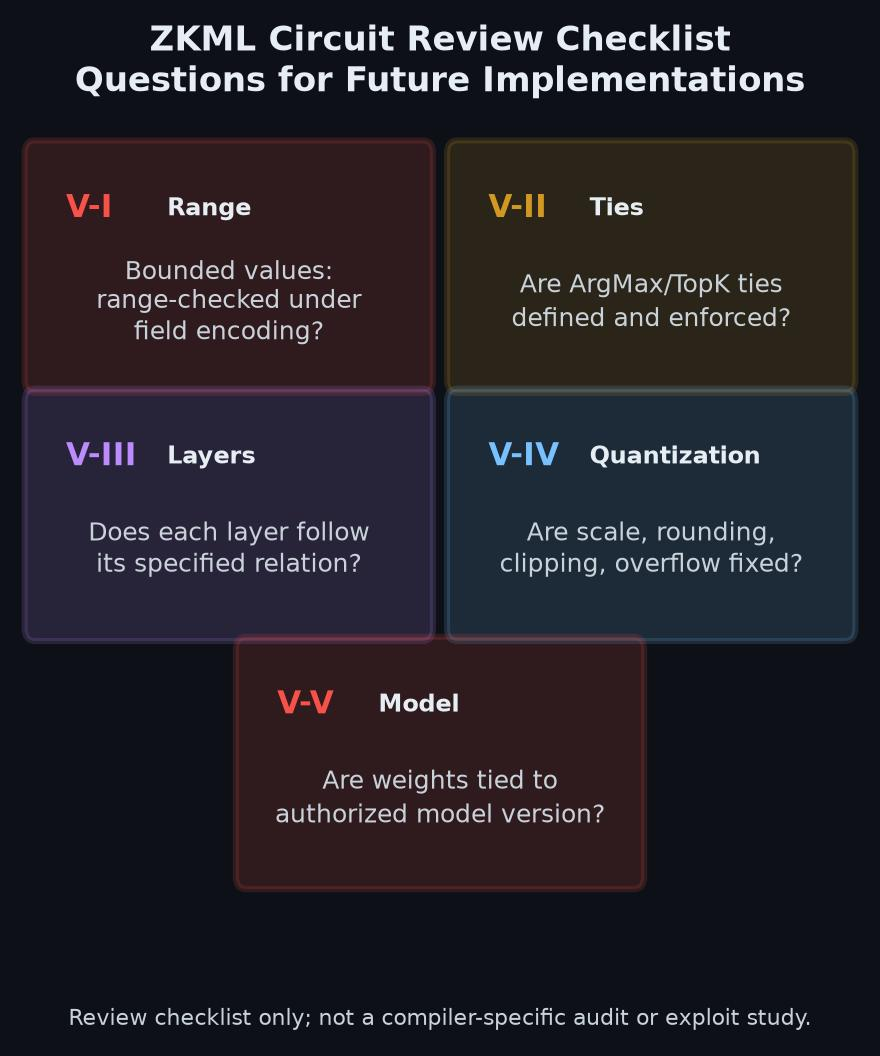
\includegraphics[width=\columnwidth]{figures/fig_zkml_taxonomy.jpg}
  \caption{Five design review questions for a future PoUI inference circuit, not a circuit audit or universal soundness requirements.}
  \label{fig:zkml_taxonomy}
\end{figure}

\textbf{V-I Range and representation.} For bounded or quantized values, check that the circuit's field-to-integer representation and range match the intended model. Use range constraints or lookups where required by the encoding; the effect of a missing constraint depends on the circuit.

\textbf{V-II Witness choice.} ArgMax and TopK outputs need defined tie semantics. Specify whether ties permit multiple valid outputs or require a deterministic tie-break, then constrain the circuit to those semantics. An arbitrary strict-margin rule may change the intended function.

\textbf{V-III Layer linkage.} If only the I/O relation is constrained, intermediate activations may be unconstrained. Require $h_{k+1}=f_k(h_k)$ for each layer, with the corresponding relation for residual paths.

\textbf{V-IV Quantization semantics.} Bind the scale, zero point, rounding, signedness, clipping, and overflow rules to the authorized model/configuration and ensure the circuit implements those rules.

\textbf{V-V Model binding.} If weights are supplied dynamically, bind them to the authorized model/version, for example through a checked commitment. If weights are fixed in the circuit, bind the circuit/version identifier to the protocol's authorized model.

Which checks apply depends on the model, encoding, and proof system. A future audit should inspect the compiled constraints, backend, quantization semantics, and model graph.

\paragraph{EZKL smoke test}
To ensure the suggested proof interface is executable, we created a deterministic ONNX model $\mathrm{Gemm}(2\times2)\to\mathrm{ReLU}$, generated a witness, then produced and verified a proof with EZKL 23.0.5. On an Intel Core i3 1005G1 laptop, proving took 6.91\,seconds, verification 27.5\,milliseconds, and the proof JSON size was 17{,}790 bytes. The test uses a locally produced SRS and a small model, making it a toolchain smoke test rather than a security or performance benchmark. The objective is to show that IC-01/IC-02 (Section~\ref{sec:codesign}) may be instantiated, but it does not validate the five checklist elements for a production compiler or model.

\section{Post Quantum Sizing}
\label{sec:pqc}

Table~\ref{tab:pqc_sizes} reports byte sizes from FIPS 204 Table~2~\cite{nistfips204}, alongside Ed25519~\cite{rfc8032} and ECDSA-P256~\cite{nistfips1865}. This is a sizing calculation, not a timing benchmark.

\begin{table}[!b]
\caption{Key and signature sizes. ML-DSA rows: FIPS 204 Table~2~\cite{nistfips204}, Ed25519: RFC 8032~\cite{rfc8032}, ECDSA-P256: 256 bit curve~\cite{nistfips1865}. Amplification is signature bytes divided by 64 (Ed25519).}
\label{tab:pqc_sizes}
\centering
\begin{tabular}{@{}lrrrrl@{}}
\toprule
Scheme & PK (B) & SK (B) & Sig (B) & Amp. & NIST? \\
\midrule
Ed25519    & 32   & 32   & 64   & $1.0\times$ & no \\
ECDSA-P256 & 64   & 32   & 64   & $1.0\times$ & no \\
ML-DSA-44  & 1312 & 2560 & 2420 & $37.8\times$ & yes \\
ML-DSA-65  & 1952 & 4032 & 3309 & $51.7\times$ & yes \\
ML-DSA-87  & 2592 & 4896 & 4627 & $72.3\times$ & yes \\
\bottomrule
\end{tabular}
\end{table}

For a 100 validator committee, one unaggregated ML-DSA-44 signature per validator totals $100\times2420=242{,}000$ bytes (about $236$\,KiB). This is a signature only payload subtotal: it excludes proofs, transaction framing, and networking, and is not a complete block size estimate. Aggregation is not implemented or measured here.

ML-KEM-768 can establish a shared secret for confidential probe delivery. Authenticated key registration is needed to bind the ML-KEM public key to a validator, and an AEAD scheme is needed to encrypt the probe. This study does not measure these operations.

\section{Layer Contracts}
\label{sec:codesign}

Figure~\ref{fig:architecture} is a requirements diagram, not a running stack. It specifies where future implementations must share data and enforce deadlines.

\begin{figure*}[!t]
  \centering
  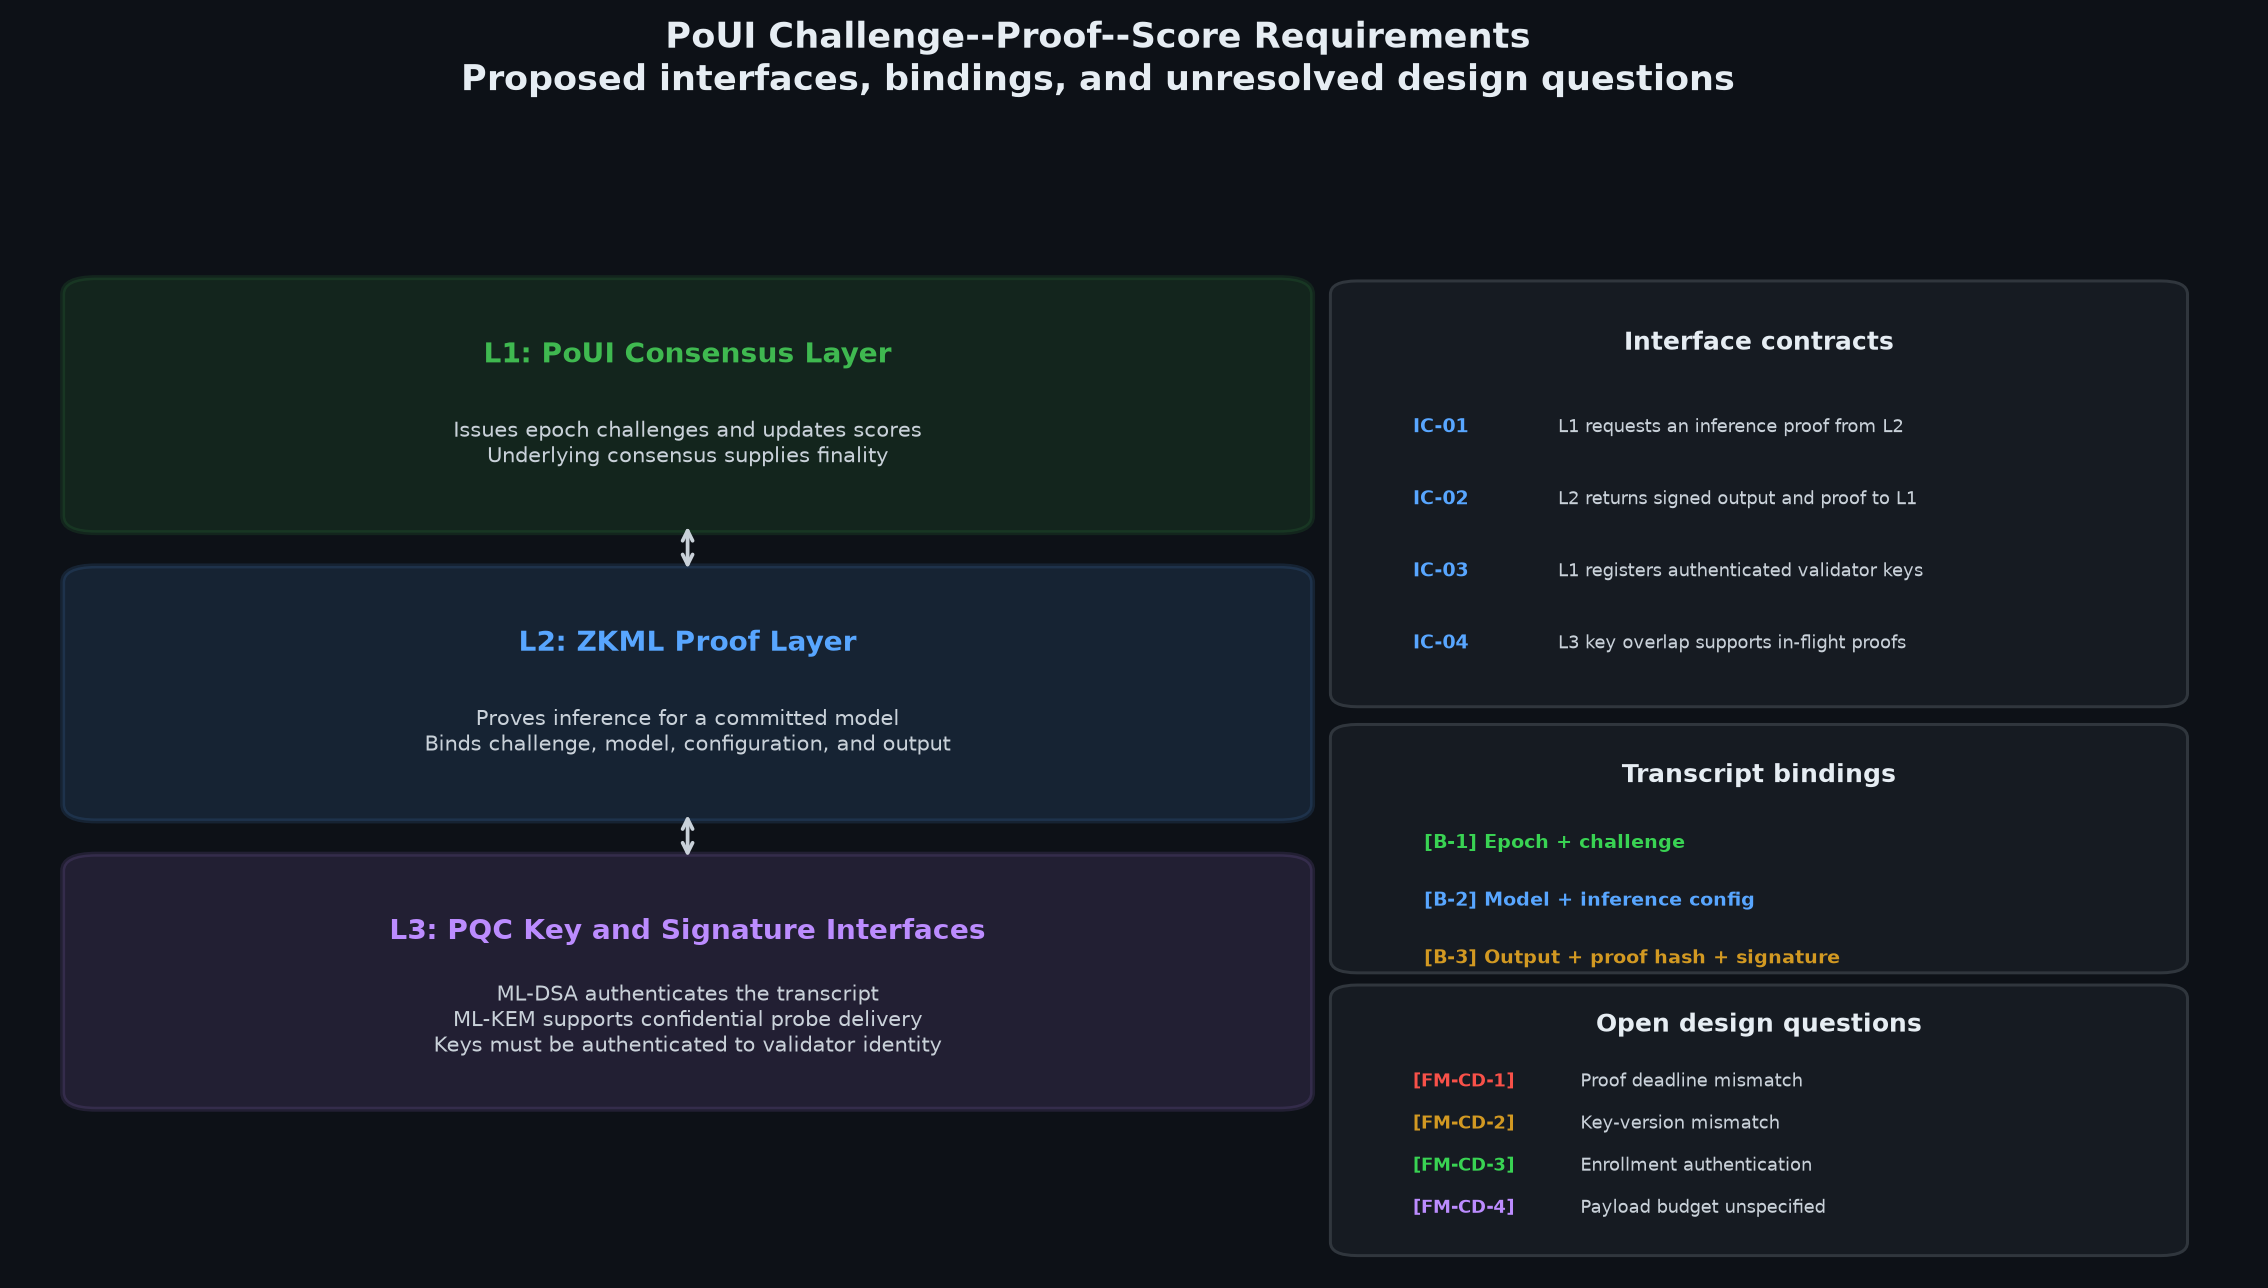
\includegraphics[width=\textwidth]{figures/fig_architecture.png}
  \caption{Proposed challenge/proof/score interfaces and unresolved design scenarios, not an implemented stack.}
  \label{fig:architecture}
\end{figure*}

IC-01 (L1$\to$L2): Request a proof of $y=f_\theta(x)$ under commitment $H(\theta)$, with an example budget of $5$ seconds and around $200$ KB.
Failures include timeout, underconstrained accept, and out of memory.

IC-02 (L2$\to$L1): submit $(y,\pi)$ with an ML-DSA signature over a domain-separated digest binding the epoch, validator identity, challenge commitment, model/configuration version, output hash, and proof hash. A verification rejection alone does not establish malicious intent or imply a slash; penalties require a separately specified evidence and appeal policy.

IC-03 (L1$\to$L3): authenticate the registration and bind ML-DSA and optional ML-KEM keys to the validator identity. ML-KEM does not authenticate a public key by itself. HNDL is a confidentiality risk for classical encryption, not for a signature channel.

IC-04 (L3$\to$L2): verification keys overlap for one epoch so that proofs initiated under key $k$ can still be checked after rotation.

Published EZKL measurements for small quantized models report proving times in seconds~\cite{ezkl2024}. A one-second BFT slot cannot wait for such a proof within the same slot. The $5$\,s budget is illustrative; a protocol should be tailored to its model and hardware. The design may require asynchronous commit-reveal, where a commitment is proposed in slot $s$ and evidence is opened later. Without a pipeline, slots may be missed (FM-CD-1); without a key-overlap window, in-flight proofs may fail during rotation (FM-CD-2). A classical-only bootstrap can compromise long-term confidentiality (FM-CD-3), while individual PQC signatures and raw proofs may exceed a block budget (FM-CD-4).


Signing a context-bound submission digest attributes those message bytes to the registered key, subject to key-management assumptions. A signature does not establish that $\mathcal{C}$ is sound or that the inference is correct. A verifier rejection alone is not sufficient evidence for slashing; the protocol needs defined evidence, false-positive handling, and appeal rules.

\section{Limitations}
\label{sec:limits}

The simulation uses $N=100$ and ten seeds. Detection is a Bernoulli trial with no honest false positives, availability is fixed at $U_t=1$, and the vote baseline is illustrative rather than a proof-of-stake model. The ZKML smoke test is limited to one device and a locally generated test SRS; it does not evaluate other EZKL, Halo2, or Groth16 configurations. Theorem~\ref{thm:game} is a one-shot result, and Lemma~\ref{lem:slash} assumes $U_t=1$. The PQC discussion uses standard byte sizes rather than locally measured cryptographic operations. These limits make the work an analytical feasibility study, not a deployment-performance evaluation.

\section{Conclusion}
\label{sec:conclusion}

This paper outlines candidate evidence requirements for a future PoUI consensus design: a defined score, a challenge/proof/score flow, a circuit that binds outputs to the prescribed model, and a specified message budget. Under the stated independent-audit model, the analysis predicts geometric exclusion, and the Monte Carlo results are consistent with that prediction. A tiny EZKL run is a toolchain smoke test, while the sensitivity calculation illustrates why false-positive handling matters. A future prototype would need to implement hidden-probe delivery, use an appropriately trusted setup or a setup-independent proof system, audit a nontrivial compiled circuit, and measure PQC operations before making end-to-end security or performance claims.


Code and figure scripts: the companion repository for this manuscript.

\bibliographystyle{IEEEtran}
\bibliography{references}

\end{document}

